\documentclass{article}
\usepackage[utf8]{inputenc}
\usepackage{hyperref}
\usepackage[margin=1.5in]{geometry}

\usepackage[makeroom]{cancel}
\usepackage{graphicx}

\usepackage{enumitem}


\title{Advisor Guide: Answers to Common Questions}
\author{ThanhVu Nguyen\\\\\href{https://roars.dev}{Roars Lab}}
\date{}

\begin{document}

\maketitle


\tableofcontents

\newpage

Adapted from \href{https://www.cs.columbia.edu/wp-content/uploads/2019/03/Get-Advisor.pdf}{this} advising guide for my 
\href{https://roars.dev}{Roars Lab}. More general PhD admission advice can be found in my \href{https://code.roars.dev/phd-cs-us/}{PhD Admission Demystify} book.


\section{Advisor Style \& Expectations}

\begin{enumerate}[label=\arabic*.]
    \item \textbf{Does the professor have tenure yet?} [engagement level, PhD might get interrupted]  
    
    Yes, I am tenured. If you are wondering if I will be around for a while, the answer is yes. Northern Virginia is a great place to live and work, and \href{https://realgmucs.github.io/stats}{CS@GMU} is growing fast and getting better every year.
    
    More importantly, having tenure allows me to take risks, pick problems I care about, and ignore the \textit{publish-or-perish} pressure that many non-tenured faculty face. That also means my students have to be independent and take initiative in their work because I won't be pushing them to do things (actually, regardless of tenure, I have always been a hands-off advisor and I expect my students to be independent).

    \item \textbf{What is the professor's formal training / background / PhD?} [helps contextualize problems/approaches]  
    
    I did my undergraduate and Master's in CS at Penn State University. Then I did my Ph.D. in CS in the University of New Mexico-Albuquerque and then a postdoc at the University of Maryland (in \href{https://plum-umd.github.io}{PLUM lab}). I started wanting to work on evolutionary computing, and then gradually changed to software engineering, programming languages, and formal methods.  Outside of academia I have worked at the Naval Research Lab and Lockheed Martin. 

    You can see my \href{https://raw.githubusercontent.com/dynaroars/latex-cv/main/cv.pdf}{CV} and other details from my \href{https://roars.dev}{lab} page and \href{https://tvn.roars.dev}{homepage}.

    \item \textbf{What have previous lab members done after getting their PhD?} [Gone to industry?/Post-doc?/Professor?]  
    
    So far I have only graduated one Ph.D. student: Guolong Zheng (2022), who is now a faculty at Minjiang University in China. Didier plans to graduate in May'26 and is applying for faculty positions.  
    
    I also graduated an MS student, who now works at Oracle, and an undergrad, who works at Jump Trading.
\end{enumerate}

\section{Group Composition \& Structure}

\begin{enumerate}[label=\arabic*.]
    \item \textbf{Do you work with undergraduate students?} [if you are an undergrad applicant]

    Yes, I work with many undergraduates over the years. Typically at any time I have 2--3 undergraduates working in the lab. 
    
    My undergrads are often supported either through research grants (e.g., NSF REU and university funding) or hourly pay. I treat my undergrads as PhD students, give them flexibility to find solutions (to projects that I give them), and push them (\emph{way}) beyond their comfort zone to realize their potential.
    
    As examples, Linhan started as an undergrad at UNL and continued as a PhD student GMU, KimHao published \emph{9 papers at top conferences and journals} as an undergrad at UNL, Stefania won the Outstanding Undergraduate Research Award at GMU, and Azan---a first year freshman when joining our lab---built \href{https://roars.dev/cspicks}{CSPicks} app within just a week of joining.

    See the \href{https://roars.dev#people}{Roars People section} for current undergrad members.

    \item \textbf{How many students are in the group?} [Number of undergrad/masters/phd/post doc]

    Check out the \href{https://roars.dev#people}{Roars People section}. Typically we have around 5 PhD students and a couple of undergrads. We have yet to have a postdoc, but my students collaborate with postdocs at other institutions, e.g., Hai works with Thanh Le at  NICT (Japan) and Guolong with Chanh Le.  We call these collaborators ``honorary'' lab members and they are very much part of our lab family.

    \item \textbf{What is the lab structure?} [how collaborative/disjointed are lab members' projects?]  

    Each student---regardless of undergrad or PhD---has projects that they lead. However, everyone is encouraged to collaborate and help each other. In weekly lab meetings, you will hear about the progress of other projects and can contribute ideas and help with problems. We also have a lab server on Discord where we chat about research and other random things.  
    
    As examples, Didier works on Complexity analysis. KimHao worked analyzing build systems, and also complexity analysis and invariant generation. Hai works on DNN verification. Linhan works on DNN testing. Hai, Linhan, and Nguyen often talk to each other as their projects involve neural networks. Long does not work with verification but contributes ideas and expertise as he knows ML systems well. And everyone contributes to fun web apps (e.g., \href{https://roars.dev/cspicks}{CSPicks} by Azan).

    \item \textbf{Do students mostly work with senior students or directly with professor?}  

    They work directly with me, but I encourage new lab members to work with senior students with similar interests.
\end{enumerate}

\section{Advising Style \& Meetings}

\begin{enumerate}[label=\arabic*.]
    \item \textbf{Does the advisor consider themselves a ``hands-on'' or ``hands-off'' advisor?}  

    I am a \textit{hands-off} advisor. Students who need a lot of guidance and hand-holding \emph{will not} enjoy working with me.  
    I will suggest directions and ideas, but I expect students to be able to work independently and take ownership of their projects. My students---including undergrads---need to be self-motivated and take initiative.  
    
    For new students, I can provide some help (e.g., directions and writing). As students become more senior/mature, I would gradually transition to a hands-off advisor. However, if I see new members capable of working independently from day one, I will let them do so from day one -- I don't get in the way of capable students. For example, below is a direct quote of what I reply on Discord to a \textit{new undergrad} student (that I found highly capable just after a couple of weeks of working together and they already built a serious working prototype) when they questions about a technical detail:
    \begin{quote}
    \textit{``I am not sure what would be best. Do what you think is best and that would be best.''}
    \end{quote}

    However, although I am hands-off most of the time, I do step in when it's really needed. If a student is truly stuck, facing an urgent problem, or approaching a deadline, I instantly switch into a very hands-on (or protector) mode. This only happens a small fraction of the time, but in those moments I will work closely with the student to get through the challenge.
    
    As mentioned, I highly encourage my students to talk to other lab members for help and guidance, e.g., more experienced students can help new students with ideas and research guidance. Our lab members are very close and collaborative: they challenge each other's ideas and help each other with problems.

    \item \textbf{How does the advisor give feedback on papers / what is their feedback style?}  
    
    For the students' first papers, I would ask for drafts and revise the draft iteratively with the students (e.g., through Overleaf). In some cases, I would rewrite most of the students' drafts, e.g., the Intro and Evaluation, for their first papers (because new students often do not know how to write these sections). This helps the students see how papers are written. Same thing with paper rebuttals, I will work with the students and revise the writing directly.  
    
    As the students have more experience, I will let go more and more. By the time the students can write and successfully publish the paper by themselves without much revision and editing from me, then I know they are ready to graduate.

    \item \textbf{Are there lab meetings? What are other meetings you will see your advisor in a group with other people?}  
    
    Yes, we meet weekly in the conference room on Thursday afternoon in the CS conference room. Everyone speaks, everyone contributes, no one is silent. Typically, the students talk about what they have been doing in the past week and what they will do next week. They also talk about issues they are facing and others contribute ideas to help solve the problems.  
   
    After status updates, a student will typically present their work in depth. The meeting usually lasts about 1–-2 hours depending on how much we have to discuss. I am usually available after the meeting to chat with students individually if they have more questions.

    Sometimes we all come and work together in a large conference room (e.g., when we are close to a paper deadline), and then have lunch together. This \href{https://photos.roars.dev/}{Google Photos album} shows some of our lab gatherings.

    \item \textbf{What does a group/lab meeting look like?} [Or other relevant meetings]  
    
    We start talking about our status, e.g., each person talks about their work for about 2-–4 mins. This is inspired by the \href{https://mwhicks1.github.io/papers/score.pdf}{SCRUM method} used in the PLUM Lab at UMD.  
    
    Then we go in depth in some topic, e.g., a student might talk about some problem they are working on, show their computation on the board, or present results. Sometimes we read papers or look at some existing tools/techniques. We plan to use about an hour for this but usually it goes beyond that. I usually have to go pick up my kids at that time, but the students want to continue and they keep going.  

    Our lab is highly collaborative and social among lab members. They often help each other with problems, which I highly encourage.  
    There are several self-identified introverts in the lab, and while they do not speak much outside the lab, they are very active and engaged in our lab meetings. This is in part because they are confident about their research and their ideas are respected by others.


    Sometimes we just relax and watch a movie (e.g., the PhD Movie).  
    
    Also, most of our communications happen on Discord server outside the meetings where we chat about research and other random things (e.g., plan for Thanksgiving party).

    \item \textbf{How often does the advisor meet with their students?} [1:1 or all together? Daily guidance by PI or post-doc?]  
    
    In addition to weekly lab meetings described above, students can talk to me individually about any thing they want (usually we would talk right after regular lab meetings). And during paper deadlines, we sometimes meet several times a day on Zoom.

    Many of my students work late at night and so do I (after kids have gone to bed!). So I've been making myself available to work with my students at night whenever they need, often 9:30 PM -- 11:30 (much later when I was younger).
    
    That said, I highly value independence, and so as long as it works for you and you're productive, it \textit{doesn't matter} to me how/when you work.


    \item \textbf{How often are students expected to be contactable by their advisor?}  
    
    Most of my communications with students happen over Discord. I sometimes contact students through email when it is something important, (e.g., the university asks me to get in touch with you about something). For such occasions, I expect you to respond to my emails quickly. However, in general, communications through Discord are more casual and you can respond when you see them --- though I find that all my students are quite responsive on Discord.


\end{enumerate}

\section{Research Fit \& Projects}

\begin{enumerate}[label=\arabic*.]
    \item \textbf{How directly applicable will your future technical skills be to the roles you want after graduating?} (If set on industry) 

    During PhD we train you to be researchers, and so if your post-graduate career is not related to research, then you are not directly using the skills you learn in the PhD. Still, many other skills that you learn---being independent, problem solving, read/write technical papers, endure my advising style, etc---are applicable to many careers.

    More specifically, skills you learn in my group (formal reasoning, verification, program analysis, being independent, writing well, etc) are real skills that are applicable to both academia, industry, and everywhere else.  We go for hard problems and they often coincide with real problems in the industry. We didn't set out to solve ``industry problems'' per se, but we often end up solving them anyway. For example, KimHao's work on build systems is directly applicable to large-scale software development at Facebook. Hai's work on DNN verification is applicable to many systems that use DNNs, which we believe will soon be everywhere (e.g., self-driving cars).

    
    \item \textbf{What research methods does the lab use?} (What \textit{types} of papers / contributions / conferences targeted)  
    
    Our work is often on developing new techniques/algorithms and building tools. We target top-tier conferences in the field (e.g., ICSE, FSE, ASE, ISSTA, OOPSLA, PLDI, CAV). For work we wish to extend, we also publish in journals such as IEEE TSE.  
    
    Ok, that was a boring neutral ``academic'' answer. The fact is that we don't just publish papers or produce boring incremental results, we also develop tools that actually work, win competitions, and receive significant awards. Our competitors are the best in the world and we enjoy \emph{beating them}. For example, \href{https://code.roars.dev/neuralsat}{NeuralSAT} is often considered one of the best at DNN verification competition and outperforms many other state-of-the-art tools.

    \item \textbf{What are some of the projects that you and your students are currently working on?}  
    
    We are working on various software analysis projects, including formalizing and proving mathematical theorems, neural network verification and inference, analysis on highly-configurable software, and program testing, analysis, and repair. 

    Ok, cross out \cancel{program repair} --- I moved on from that. Nowadays I am more interested in DNN verification and reasoning and also using LLM-based proof assistants to formalize and prove mathematics.

    \item \textbf{In general, do you tend to give your students projects or have them select their own?}  
    
    I give them research topics or directions to explore. For new students, usually, I give them more specific projects to start with so they can get familiar with the research area and techniques. As they are more familiar, they will be able to come up with their own projects. For example, Linhan bounces around several ideas before settling on his work on DNN benchmarking, and Hai and Long work with several students (some not even in our lab) on various projects.
    
   I also aim to determine what my students are good at, and then help them find projects that fit their interests and strengths. This is not just for research, but also for other things. E.g., in our Thanksgiving party, which I host at my house every year for my lab and their families, I delegate tasks to students based on their strengths and interests: I found out that Linhan is very good at cooking, so I appointed him as our turkey ``czar'' responsible for a 20+ lb turkey roasting for 30 people!

 
    \item \textbf{Do you have particular projects that you see me working on?}  
    
    It depends on your background and interests, but I do have many ideas to try. In recent years, I have been focusing more on DNN reasoning and verification, so something related to that.   
    

    \item \textbf{How much freedom do you think I'd have in selecting my own projects?}  
    
    We need to find projects or research directions that we are both interested in. Once we have agreed on a research direction you will have a lot of freedom to explore and develop your own projects. 

    However, if you want to work on some areas that I am not interested in, then I would rather you find another faculty because I can't guide a topic I don't know or care about.

    That said, I am open to new ideas \emph{if} you can convince me you can make them work. The best way to do that is as follows: if you come up with an idea that is quite different than what you're working on, \emph{DO NOT} tell me about it, especially if you don't have good things to back it up, because I will likely shoot it down. Instead, just pursue it (while still working on your main project), and build \emph{a prototype} and achieve some \emph{good results}. If you can show me your ideas work with concrete results, I will much more open to them. This happens multiple times in my lab, and probably some my students are currently working on secret ideas that I don't know about yet!

    \item \textbf{Are there other students you are interested in working with? If so, what would they be working on project-wise?}  
    
    Not sure what ``other students'' means.

    \item \textbf{Would they have their own line of work or contribute to a bigger project/someone else's project?}  
    
    All of my students have their own line of work.  They also collaborate with other lab members and in the beginning, they likely work on projects with other students. But eventually, they will \textit{own} their projects.
\end{enumerate}

\section{Expectations \& Progress}

\begin{enumerate}[label=\arabic*.]
    \item \textbf{What progress does the advisor generally expect from a student in the course of a semester?} [Submission/Publication pace]  
    
    I expect the student to have enough results that they can \textbf{submit} a paper to one of the top conferences each year. It does not have to be accepted because the reviewing could be noisy, but it is crucial to complete the work and submit it. 
    
    You can see how my students publish in the \href{https://roars.dev#publications}{Roars Publications section}. % and also \href{https://github.com/dynaroars/dynaroars.github.io/wiki/Collaborators}{this collaborator page}.

    \item \textbf{What other expectations does the advisor have for their students: time, vacation, paper, project,experiment wise etc.?}

    I want you to \textit{be independent} and \textit{take initiative} in your work. Don't just wait for me to tell you what to do. If you have an idea, try it out yourself and show me the results.
    
    You will have \textit{freedom to come up with solutions and explore ideas in your own way}. Your projects need to be related to my interest, but beyond that, you can do things your way.  
    
    I want you to \textit{ask questions} and \textit{be open to learning new things from others} (e.g., your lab mates, who are probably better resources to learn from than me).  
    
    I want you to listen to me, but also \textit{be independent} and \textit{challenge me}. I am not always right but for you to challenge me, you must be able to convince me, through concrete evidence and results, that your idea is better than mine. 
    
    As an example, if I tell you to try \textit{X}, but you think \textit{Y} is better, then you should do both \textit{X} and \textit{Y} and show me both results. It doesn't matter if \textit{X} or \textit{Y} is better, but that you believe in your idea and can get results to support it.

    \item \textbf{When have you given a letter of concern? Why?}  
    
    I haven't given a letter of concern yet, and I hope I never have to.  
    But I'd remind and warn the student if they need to be on track or do not meet the expectation. 
    
    Here is the expected progress for my Ph.D. student. By the end of the second year, you should publish at least a second-author paper. You are doing well if you publish a first-author paper at that time. By the end of the third year, you are considered behind if you do not publish a first-author paper and are seriously behind if no good submissions were made. A typical student in SE/PL will have 4--5 publications, my students often have a lot more than that.
\end{enumerate}

\section{Funding \& Obligations}

\begin{enumerate}[label=\arabic*.]
    \item \textbf{Where does their funding primarily come from?} [If military/industry-focused funding bothers you, figure this out]  
    
    Most of my funding sources are from NSF and some are from the industry (e.g., gifts from Amazon and Facebook). All of my funded projects are on basic/fundamental scientific research.

    \item \textbf{What are their constraints from their funding source?} [Some restrict research topic and change final deliverables. Some add work — writing progress reports, traveling, preparing presentations for the funding source or engineering overhead for integration]  
    
    Since my funding sources are mainly from NSF or unrestricted from industry, our work has few constraints. Occasionally, I may need your assistance on progress reports and presentations if you are funded through specific grants.

    \item \textbf{If your advisor made you work on a project in their area that you are least interested in (e.g., for a grant) would you still be excited doing work?} [Useful for choosing between advisors]  
    
    It is unlikely that you have to work on something you're not interested in.

    \item \textbf{If you run out of your primary funding for a student how do you expect the student to handle that?} [advisor's responsibility / you'll have to write a grant with me / dept will cover the student / you have to find their own funding]  
    
    One of my responsibilities is finding funding to support my students, and I have been quite lucky to have sufficient funding to support my students (including summer). However, as a fallback, the department can also cover the student with TA-ship. \href{https://github.com/dynaroars/dynaroars.github.io/wiki/About-GMU}{CS@GMU} is \textit{very good} at providing Ph.D. students TA-ships.

    I also encourage my students to apply for fellowships. I will help them with the applications (e.g., give feedback on your statements and provide LORs). These fellowships are not necessary for funding, but they are prestigious and can help your career. I take pride in my students' achievements---sometimes more than in my own. When a student wins a fellowship or an award, it's also a win for me and the entire lab!
\end{enumerate}

\section{Program Requirements}

\begin{enumerate}[label=\arabic*.]
    \item \textbf{What does the quals process look like?}  
    
    The department has a very specific guideline and timeline that students need to follow for the comprehensive exam. It's quite straightforward and the student needs to write a paper describing the research area and problem they want to work on and present that paper. After the comps, they need to form a dissertation committee, and then do a proposal defense and finally a dissertation defense. The department provides clear guidelines on all these steps.

    \item \textbf{Is there a TA requirement? / How often would I be expected to TA?}

    There is no TA requirement from the university or the department. Nevertheless, I strongly recommend doing a TA at least once or twice during your PhD. TA is a great way to get introduced to teaching, and can really help if you're interested in an academic career. More practically, in some cases not having to support you as a GRA during the normal Spring/Fall semesters would allow me to support you during the Summer.
\end{enumerate}

\section{Recruitment \& Fit / Placement}\label{sec:recruitment}

\begin{enumerate}[label=\arabic*.]
    \item \textbf{Are you taking a student? Do you have funding to take students in this year (or, for which projects)?}  
    
    I am \emph{not} actively recruiting (my lab already has quite a few students), but I am always looking out for \emph{standout} students. Standing out is difficult to define and subjective---I can only know it when I see it (e.g., see the Reddit example in~\autoref{q:a-scrapper}).

    \item \label{q:a-scrapper} \textbf{What factors will affect whether or not you take a student?}  
    
    Here's a concrete example: One day the CS faculty were talking about a GMU Reddit post from a student who built a web app to identify ``easy A'' classes at GMU (because they find RateMyProfessors not useful). Some profs. found it problematic because this app allows students to find and take easy classes (and they also complained that it doesn't represent their own classes fairly). But I was intrigued.  
    
    I didn't care much about the app itself, but the initiative and technical skill caught my attention: the student finds a problem, comes up with a solution using an unconventional way (from publicly available FOIA data that no one pays attention to), and implements an app that attracts many students (and upset professors!).
    
    That same evening, I mentioned the app on our lab Discord server (\autoref{fig:ascrapper}), and we determined the developer's identity by analyzing the code and deployment details. I emailed the individual right after, we talked the next day, he was very interested in our research, and so I hired him on the spot.

    \begin{figure}
        \centering
        
\includegraphics[width=0.7\textwidth]{files/ascrapper.png}
        \caption{Recruiting the ``A scrapper student''.}\label{fig:ascrapper}
    \end{figure}


    \item{Do you think our research interests are a good match?}
    
    The question should be: are \emph{my} research interests a good match for \emph{you}? As mentioned, I will unlikely work on something that I am not interested in. So if you want to work with me, you need to be interested in \href{https://roars.dev}{my research areas}. 

    \item I'm interested in working with you. Do you think I'd have a good chance of working with you if I come to your university?

    If you come to GMU and want to work with me, let's chat. However, the \emph{best} way for me to know you (and vice versa) is taking my classes, being stand out, and impressing me. I recruit several students (e.g., Linhan, Guolong, and Didier) from my classes that way.

\end{enumerate}

\section{Co-Advising \& External Collaborations}

\begin{enumerate}[label=\arabic*.]
    \item \textbf{Would the advisor be interested in co-advising?}  
    
    I was co-advised during my PhD and it worked out, but I \textbf{prefer to be your main or sole advisor}, and other faculty members can be collaborators (but not co-advisor). This way, you can get more attention from me while still being mentored by other experts. For example, Hai is advised by me but also collaborates (and therefore mentored) by Matt Dwyer at UVA through our NeuralSAT project. It's also easier for me because I do not want to deal with conflicts between co-advisors, e.g., if they want you to do something that I don't want you to do (and vice versa).

    In addition, I am \emph{not} into broad \emph{interdisciplinary research}, which would be beneficial for co-advising. I prefer to work on problems in my fields of SE/PL/FM and related ones (e.g., logics, mathematical proofs). So if you want to do interdisciplinary research in areas outside my core expertise (e.g., CS + Bio), then I may not be the best fit for you. While interdisciplinary work has many values (and I admire people who do it well), I have determined that it is not my strength and I prefer to focus on my core areas.

    If you'd like to do interdisciplinary work that I am not too interested then I would not want to be your main advisor. I would rather you find another faculty member who is more interested in your work and can help you with it, (e.g., the \href{https://roars.dev/cspicks}{CSPicks} tool can help explore faculty interests). I think this is a better fit for both of us.

    \item \textbf{How do you handle it when a student outgrows your expertise — they know more than you?}  
    
    I \emph{expect} this to happen. At some point, my students will know more than me in their topic of interest. Depending on the projects, I may introduce my students to people who are experts in that area and together we can collaborate with them. For example, KimHao works with Quoc-Sang at Facebook on build systems, and Hai works with Matt Dwyer at UVA on DNN verification. In short, if you become better than me in your area, then I've done my job and you're ready to graduate.  
    
    Note that if you want to change or try another research direction that I don't have much expertise or interest in, then I can't help you much there then we may need to discuss switching advisors. This is common in academia (almost happened to me during my PhD) and I have no issue with you doing that (in fact, some of my students came to me after switching from other advisors).

\end{enumerate}

\section{Lab Resources \& Working Environment}

\begin{enumerate}[label=\arabic*.]
    \item \textbf{What equipment are provided to students?}  
    
    I purchase computers and electronics for my students (e.g., computers, laptops, monitors, hard drives, memory, headsets, keyboards, etc). Our lab has several \href{https://github.com/dynaroars/dynaroars.github.io/wiki/Servers}{powerful servers} such as Nvidia Spark DGX (a gift from NVidia), that are shared among the students.  
    Let me put it this way: our lab machines are much better than most other labs and our experiments get done much faster than others.

    \item \textbf{Do students work together in common space? Do students often get meals together?}  
    
    Sort of. Due to office space limitations, my students are sharing space with other SWE PhD students. There are advantages of that as you get to interact with more people outside our lab.

    \item \textbf{Do students often work late?} [Often / only before conference deadlines.]  
    
    We work late mostly before the conference deadline. I also stay up quite late to chat with students if they need. Though it really does not matter to me when you work as long as you are productive.

    Work-life balance is a strange thing in CS research. During paper deadlines, we work very hard and long hours---and I do expect my students who are involved in the paper to do so as well. But outside of deadlines, we have a lot of flexibility, e.g., feel lazy and want to take a break for several days? No problem. I don't care and you don't even have to tell me (in fact, you should not tell me!). In short, creativity comes from freedom and flexibility, and in this regard, I give my students a lot of freedom.



    \item \textbf{Are there snacks in the lab?}  
    
    Not sure, sometimes I see some snacks. When I was a grad student, I often stole pizza and food from other labs (I have plenty of stories to tell). I often take my groups out to eat (e.g., when working on papers, or end-of-semester gatherings, in fact, I am writing this while preparing for traditional lab Thanksgiving dinner).  
    
    More generally, we work hard but also have \href{https://photos.google.com/share/AF1QipNMHIvnSmq5bjer6I6r1Ddb4yiBt3jgq4yrA7q5lSmo4ePHfmiXhXqhk8IhKf47lA?key=SkJhMjZtYmoyT1Q2aW1ERGpRa2VTclZrbzJVLUpR}{lots of fun}, many of which involve eating and gathering.
\end{enumerate}

\section{Conferences, Travel \& Internships}

\begin{enumerate}[label=\arabic*.]
    \item \textbf{How often do grad students get to attend conferences?} [Pace + What constraints]  
    
    If you have a paper at a conference, even not as first author, I will support your travel to the conference to present it. I also encourage you and other lab members to go to local conferences or workshops (e.g., PL meetings at schools in the Northeast region such as Stevens, Princeton, UPenn). I often send my students to the annual, week-long Formal Techniques Summer School in San Francisco (CA).
    
    For full disclosure, I am not a big fan of attending conferences. I think they are useful but I am just not into traveling. I rather stay at home and play with my kids and work on my research. But this is just me and I wholeheartedly support my students to attend conferences. %Moreover, while I don't travel often and therefore cannot introduce my students to many people in person, I introduce them to researchers through emails and collaboration.

    \item \textbf{How many conferences are students expected to target a year?} [remember pubs $\neq$ submissions]  
    
    On the second year, I expect my students to \textit{submit} \textit{one} first-author paper to a \textit{major} \href{https://roars.dev/csconfs}{conference} each year (e.g., ICSE, FSE, ASE, ISSTA, PLDI, OOPSLA, CAV). 
    On the third year onwards, I expect you to \textit{submit} at least \textit{two} papers each year.

    Essentially, I expect you to get some results to present after a full year of research, and continue and improve that pace throughout your PhD.

    My students often publish more than what was mentioned above, e.g., KimHao published 9 papers as an undergrad, Guolong published 8 papers during his PhD, and Hai already has 5 papers by his 3rd year, etc. 
    
    I strongly believe that students do not know what they are capable of until they push themselves, and they should not remain in their comfort zone (not the level of craziness of \href{https://davidgoggins.com/}{David Goggins}).

    \item \textbf{Is the professor in an 80/20 with a company? Are students' research projects tied to industry funding?}  
    
    No, but I collaborate with researchers from the industry (e.g., Facebook) and have industrial grants/awards (e.g., Amazon). Some students' projects are directly applicable to industrial problems, and they get opportunities to do internships at cool companies.

    \item \textbf{Will it be acceptable/encouraged to intern at a company during the summer?} [Does this change with seniority?]  
    
    Definitely, in fact I encourage you to do that. E.g., KimHao works at Facebook (twice) during the summer. However, as PhD students, you should do research internships (e.g., at research labs in the industry) rather than engineering internships. Best if you can do something that is related to your research and can lead to publications and things you can use to support your dissertation. But if you want to do an engineering internship, I will support you as well.

\end{enumerate}

\section{Culture, Time Off \& Social Life}

\begin{enumerate}[label=\arabic*.]
    \item \textbf{How often do students take time off? Are there lab/department outings/events?}  
    
    \textbf{Time off:} Academia is flexible and I am flexible with my students (as long as they get their work done).
    However I expect my students to be in the lab at least 3 days a week (part of school requirement otherwise they will lose their space, which I think is fair).  But if they need to take time off (e.g., health appointments, personal/family events), they can always tell me and take some time off.  
    
    \textbf{Lab dinner/gathering:} Usually twice a semester (e.g., \href{https://photos.google.com/share/AF1QipNMHIvnSmq5bjer6I6r1Ddb4yiBt3jgq4yrA7q5lSmo4ePHfmiXhXqhk8IhKf47lA?key=SkJhMjZtYmoyT1Q2aW1ERGpRa2VTclZrbzJVLUpR}{group gathering} at the beginning and the end of a semester and during Thanksgiving). Once a year we also hang out with other labs at Round One (bowling and arcade).  
    
    \textbf{Department outings/events:} There are various events throughout the semester in both the SWE group and the department. I highly encourage my students to attend these to have fun and know other people.
\end{enumerate}

\section{Support, Conflicts \& Student Well-Being}

\begin{enumerate}[label=\arabic*.]
    \item \textbf{If one of your students is being treated unfairly — by a collaborator, committee member, or even within the department — how do you handle it?}  
    
    I am very protective of my students. I can be hard on them when they do research with me, but I will stand up for them. Not only obvious cases like unfair treatment but also when I feel they need support, e.g., I would shield them from being overworked or being taken advantage of by others. My priority is the well-being of my students.

    \item \textbf{How do you deal with students who are struggling? Do you ``let go'' of students who are not making progress?}  
    
    I have never let go of a PhD student yet, and I hope I never have to. Once I take in a PhD student, I see it as my responsibility to get them through the program and into a good career (job that they like).  
    
    Every PhD student will struggle at some point, but I believe my students are capable of pushing through challenges, and I will work with them to make sure that happens. So no, I don't give up on students easily. It's usually easier for them to give up than it is for me to give up on them.
\end{enumerate}


\section{Additional Questions to Understand the Advisor}

Questions that are not categorized into the above sections but can help you understand my advising style and philosophy.


\begin{enumerate}[label=\arabic*.]
    \item\label{q:scooping} \textbf{What do you think about safeguarding ideas and results so that they don't get scooped?}
    
    We have so many ideas, so if someone wants to steal some of them, it's not a big deal, and in fact, we should be be amused, flattered, and consider it a compliment! 

    Ideas are meant to be executed. If we fail to execute the ideas, then we are the one to be blamed, not the ones who take the ideas and execute them.  If the ideas are ours then we want to quickly realize them, publish them, and get the credit for them. If we don't/can't get something to work, we might as well give them to others.  And they can acknowledge us if they want -- or not (doesn't matter to me).  

    I encourage my students that if people---even our competitors in the same research area---are interested or curious about our work, tell them all; no need to hide the ``secrets'' sauce or whatever important. Give people details, point them to our code base, e.g., \href{https://code.roars.dev}{project repos}, which are always open-source and publicly available, to see all the cool things we're doing. And if they want some code or benchmarks etc, help them out and encourage them to use our work and even build on top of it.

    Of course, this might clash with collaborators, funding sources, or projects that have restrictions on sharing. In those cases, we will follow the rules and restrictions, but I will not be happy about it, and so in general would avoid such collaborations or projects. So far our projects, even those with industry collaborators, are all open-source and publicly available.

       
    
% LLMs: "How do you use LLMs in your own research workflow?"
% Taking chances on students: "What's your tolerance for risk when admitting a student — how often do you expect it not to work out, and do you do it anyway?"
% Co-authorship: "If someone contributes just 1% of a paper but it's the 1% you couldn't do yourself, do they deserve co-authorship?"
% Co-authors using work independently: "If a co-author takes your shared work and runs with it in a completely new direction without involving you, how do you feel about that?"

    \item \textbf{What do you think about course work and grades when evaluating prospective PhD students? If these are not important then what do you look for instead?}

    In my \href{https://code.roars.dev/phd-cs-us/}{PhD Admission Demystifying} book, I emphasize that for CS PhD admission good GPA rarely matters (you can read more about that in the guideline). There are much more reliable indicators of a student's potential for research; LoRs and research experience/publications of course, but even small things that seemingly unrelated to research can be good indicators, e.g., the A scrapper example in~\autoref{q:a-scrapper} or someone who climbed the Himalayas!  It doesn't have to be crazy thing (though it can be), but should be something that shows the student is a self-starter, has initiative, and can get things done. 

    \autoref{fig:stefania} is a snippet from a LoR I wrote for my undergrad student to nominate her for an Outstanding Undergrad award. At that moment, she has not done much research, but her volunteer activities show self-motivation and initiative, and that impressed me that I hired her to be my ugrad researcher and then later nominated her for the award.
    Note that the last sentence is a bit of self-deprecating humor: her pure altruistic work puts her in a different league, one that even NSF CAREER recipients, including myself, feel inadequate. The award committee apparently agreed, as she won out of many nominees.

    \begin{figure}
        \centering
        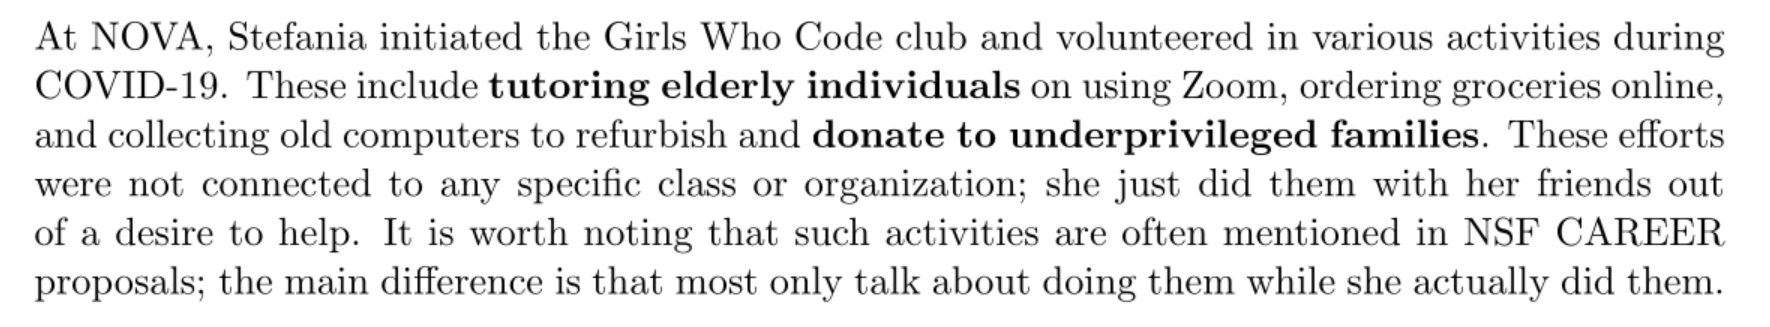
\includegraphics[width=1\textwidth]{files/stefania.png}
        \caption{Stefania's LoR.}\label{fig:stefania}
    \end{figure}
    
            
    I would go further and say if even at the admission level GPA is not that important then during the PhD it is even less important.  I rarely ask about course work and grades from my PhD students.  In fact, if they are not doing well in research but doing very well in course work, then I would question that as that can be a sign of them struggling in research and using course work as a way of coping or just trying to get by.  In short, if you're my PhD student and you get 4.0 GPA in your classes, then I might question why you spend so much time on coursework instead of research. Just do enough to get by course work and focus on research.


    %using LLM and stuff -- I do, but completely in the loop

    %taking chances with students:  1/10 is good -- do it anyway.  

    \item \textbf{If someone contributes little to a paper, do they deserve co-authorship?}
    
    ``Little'' is subjective!  We don't seek co-authors to help with our work, but if it happens that someone can help make the work better, we will share the credits. Even if we did 99\% of the work, but can't do the other 1\%, and someone else can help with that 1\%, then we should give them co-authorship. The person who did most of the work is still the first author, etc.  The point is that if we can't ship the work without that 1\%, then that 1\% is highly important and deserves co-authorship.  Thus, it's not about giving co-authorship to someone who contributed a little, but rather about giving co-authorship to someone who contributed something that we can't do ourselves that is necessary to ship the work.

    In addition, as co-author, the person can claim the work is theirs and do whatever they want with it -- and doesn't need to include or involve us at all.  We don't care about that.  We just want to do good work and get it out. In fact, if they use it and talk a lot about it, that's great---free advertisement for us.  And if they completely ``steal'' it, we should be flattered and consider it a compliment (\autoref{q:scooping})!

    \item \label{q:feedback}\textbf{Do we submit papers to see what the community thinks and get feedback}
    
    \textbf{No}, we only submit papers that we think are good. We don't send out ``feelers'' to see if the community likes our work.   We  should not use the volunteering reviewers as guinea pigs to test our work (besides, the comments from a couple of reviewers do not represent the ``community''). Moreover, we don't need to send out papers just to get feedback---I can give you feedback and you can also get them from your lab mates.
    
    If we do enough homework we should have a good idea of how the community would react to our work. In fact, if our work is so good, we can change the community's mind and get them to like it. So just do the work, get good results, then write a good paper about it.  
        
    \item \textbf{How do you approach rebuttals? Strategy?} [Do you respond to every reviewer comment, even unreasonable ones? How do you handle clearly incorrect reviews?]
    
    If the reviewers are very negative (e.g., not even a borderline), we should just \textbf{withdraw the paper}. This saves both ours and the reviewers' time. Note that even if we withdraw, we should put a note to \textbf{thank the reviewers for their time and feedback} and say that we will withdraw the paper and try to address the concerns in the future. I am adamant about this---whether we find the feedback useful or completely garbage, we will acknowledge and thank the reviewers for their time and feedback.


    However, our papers are typically not so bad that everyone hates them (i.e., we don't submit papers when they are not ready as mentioned in~\autoref{q:feedback}), so we get to do a rebuttal. My students, especially the main author(s), will draft the rebuttal (usually on shared Google Docs), and I will give feedback and revise the writing. There are many good practices (e.g., don't over-promise, don't be defensive, etc). But the most important thing is to treat rebuttal as an opportunity to improve the paper, and not to worry about the outcome or trying to please the reviewers.

\begin{itemize}
    \item \textbf{Always acknowledge} the reviewers' time and feedback, even if you think they are unreasonable or won't care (most likely they don't), but we need to do it because it's the right thing to do--even if we really hate their questions and believe nothing will change their mind.
    
    \item \textbf{Don't do the rebuttal when we are emotionally upset (e.g., after reading the reviews)}. Take a break, calm down, and then come back to it. The comments---no matter how bad they initially seem---typically have some truths in them (e.g., if they ask a really ``dumb'' basic question, this could be because we assume too much and don't explain things well enough; if they don't like the problem, then may be because we didn't motivate it well enough or we submitted to the wrong venue, etc).


    \item \textbf{Don't try to find the champion and the defectors} This is a very common strategy---find the reviewers who clearly like the paper and provide them with the ammunition to fight against the defectors.  I personally don't find this useful because, as mentioned, even the most negative comments have some truths in them and therefore can help improve the paper. Moreover, while a reviewer might appear to be strongly for or against the paper, they might actually be the opposite (e.g., a champion might not actually do anything to help the paper while a defector who is open to changing their mind if we can address their concerns).  So just address the comments with the purpose to improve the paper, and don't worry about who is a champion or a defector.

\end{itemize}
In short, treat rebuttal as an opportunity to improve our writing and work (think of them as \emph{bug reports} that make your code better), and don't worry about the rest.
In most cases, especially at top confs., papers will get rejected; and in such cases we improve and resubmit and get best paper award, e.g., our compositional verification work was rejected at CAV'25 and get Research Spotlight Award at NeurIPS'25. In some rare cases, however, rebuttal can actually change reviewers' mind as shown in~\autoref{fig:rebuttal} and we celebrate!
    
\begin{figure}
        \centering
        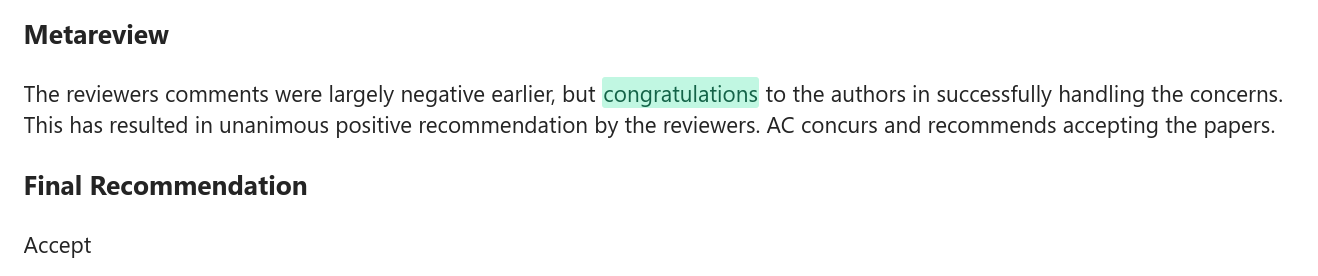
\includegraphics[width=0.8\textwidth]{files/cvpr-acceptance.png}
        \caption{CPVR'26 paper that got accepted even with largely negative reviews but a very positive rebuttal.}\label{fig:rebuttal}
\end{figure}
\end{enumerate}

    

\section{Similar Resources}

\begin{itemize}
    \item \href{https://jbhuang0604.github.io/advisor_guide.html}{Jia-Bin Huang's answers}
    \item \href{https://ideal.umd.edu/blog/Prospective-Students-FAQ}{IDEAL Lab's answers}
\end{itemize}





% 20. **How do you approach rebuttals? Defensive or strategic?**

% 21. **Do you respond to every reviewer comment, even unreasonable ones?**

% 22. **How do you handle clearly incorrect reviews?**

% 23. **What do you expect from students during rebuttal week?**

% 24. **How do you decide whether to revise-and-resubmit or pivot the project?**

% 25. **How do you emotionally handle rejection, and what do you expect from students?**

% 26. **When a paper is rejected, how quickly should we resubmit elsewhere?**

% ---

% ## Collaboration & Authorship

% 27. **How do you determine authorship order?**

% 28. **What qualifies someone to be a co-author?**

% 29. **Is it acceptable to collaborate outside the lab?**

% 30. **How do you handle conflicts about contribution or authorship?**

% 31. **Do you encourage cross-lab or cross-university collaboration?**

% 32. **What do you expect from a first author vs. a co-author?**

% ---

% ## Research Ethics & Integrity

% 33. **How do you ensure experiments are reproducible?**
% 34. **What are your expectations about code release?**

% 35. **What is unacceptable behavior in research?**

% 36. **How do you handle mistakes discovered after submission?**

% 37. **What is your policy on “salami slicing” results?**

% ---

% ## Growth Through Publishing

% 38. **When do you consider a student “ready” to lead a paper independently?**

% 39. **At what point should a PhD student stop needing heavy editing from you?**

% 40. **How do publications relate to graduation timing?**

% 41. **Do you expect students to mentor juniors on papers?**

% 42. **What separates students who publish a lot from those who struggle?**

% ---

% ## High-Level Philosophy

% 43. **Are publications the goal, or a byproduct?**

% 44. **What matters more: acceptance rate or research quality?**

% 45. **Would you rather submit a risky idea or a safe incremental one?**

% 46. **What does “beating the competition” mean in practice?**

% 47. **What kind of researcher do you want your students to become?**



% \subsubsection{Do you mainly publish in SE/PL venues or also in other areas? How do you decide where to submit to?}
% - be strategic
% - sometimes better to submit to workshop etc
% 

%\subsubsection{How do we deal with rebuttals? Do you work with students on rebuttals?}

% turn negativity into positivity (by showing the reviewers we take their comments seriously and we can address their concerns with some additional experiments or analysis). I will work with students on rebuttals and revise the writing directly.

%\subsubsection{How do we deal with paper rejections? How do we improve the paper based on reviews?}
%- not always have to listen to reviewers -- unlikely you will get the same reviewers again.
\end{document}


- qualifer exam  
- related work, taking classes to prepare 
- bandits

    
    %\item \textbf{Don't be defensive} As mentioned, it's usually \emph{something} that our paper says (or not says) that triggers the reviewers' comments, and so there's always something we can improve (regardless if it is accepted or not). So we should not try to hard to argue why the reviewer is wrong or why they don't understand, but rather try to understand why they ask the question and how we can improve the writing/work to address their concerns.  If we think they miss something, clarify; if they are asking for too much, say so and justify why we think what we have is already good enough. We don't need please the reviewers or try to change the outcome, but to improve the paper and the work.
    
    %\item \textbf{Don't overpromise} Improve writing, adding figures, better motivation, etc: these are things we can promise to do. But if the reviewer asks for something that might require additional experiments or comparison with other tools, do not promise to do these!  The reason is simple: we might not be able to do these things (e.g., the existing tools might not be available, our experiments might not work, etc). As reviewers, when I see a rebuttal that promises to do something that is not guaranteed, I'd be skeptical about it. In addition, many confs. explicitly say that they will not consider additional experiments or comparisons that are not in the original submission.